\documentclass[specialist,subf,href,colorlinks=true,14pt
%,fixint=false
,times,mtpro,specialist
]{disser}
\usepackage[
  a4paper, mag=1000, includefoot,
  left=3cm, right=1.5cm, top=2cm, bottom=2cm, headsep=1cm, footskip=1cm
]{geometry}
\usepackage[T2A]{fontenc}
\usepackage[utf8]{inputenc}
\usepackage[english,russian]{babel}
\usepackage{graphicx}
\ifpdf\usepackage{epstopdf}\fi
\sloppy

\usepackage{cite,enumerate,float}

\usepackage{vmargin}
\usepackage{indentfirst}
\usepackage[T2A]{fontenc}
\usepackage{graphics}
\usepackage{amsthm}
\usepackage{amsbsy}
\usepackage{amsmath}
\usepackage{amssymb}
\usepackage{amsfonts}
\usepackage{mathtext}
\usepackage{hhline}
\usepackage{longtable}
\usepackage{fancybox,fancyhdr} 
\usepackage{setspace}
%\usepackage{mathtext}
%\usepackage{mathenv}
%\usepackage{array}
%\usepackage{xcolor}
%\usepackage{float}
%\parindent = 30pt
%\hoffset = 12pt
%\voffset = 0pt
%\oddsidemargin = 0pt
%\evensidemargin = 0pt
%\topmargin = 9pt
%\headheight = 0pt
%\headsep = 24pt
%\textheight = 650pt
%\textwidth = 450pt
%\marginparsep = 0pt
%\marginparwidth = 9pt
%\footskip = 30pt

\begin{document}

%
% Титульный лист на русском языке
%

% Название организации
\institution{Федеральное босударственное бюджетное образовательное учреждение высшего образования <<Московский Государственный Университет им.\,М.\,В.\,Ломоносова>>\\
Механико-математический факультет\\
Кафедра вычислительной математики\\}

\title{Курсовая работа}

% Тема
\topic{<<Реализация библиотеки параллельной записи больших файлов с вещественными числами в текстовом представлении>>\\
<<Implementing of a parallel record library of large files with floating-point numbers in a text representation>>}

% Группа
\group{Студентки 410 группы}
% Автор
\author{Нагорных Яны Валерьевны}

% Научный руководитель
\sa       {К.\,Ю.~Богачев}
\sastatus {д.\,ф.-м.\,н., доцент}


% Город и год
\city{Москва}
\date{2018}

\maketitle

%\renewcommand{\contentsname}{Содержание}
\tableofcontents

\renewcommand{\figurename}{Рисунок}
\newcommand{\class}{\textcolor[rgb]{0.5,0,0.5}}
\newcommand{\type}{\textcolor[rgb]{0.5,0.5,0}}
\newcommand{\field}{\textcolor[rgb]{0.5,0,0}}

\newpage

\section*{Введение}
\addcontentsline{toc}{section}{Введение}
\paragraph{Постановка проблемы.}
Печать большив массивов чисел без округления с большой точностью всегда занимает много времени.
Однако, не вся печать упирается в возможности диска, как это может показаться.

Кроме того, у печати данных мало ресурсов для ускорения.

Печать чисел с плавающей точкой также является проблемой, так как само значение числа и его экспоненту нельзя обрабатывать независимо. 

Стандартный подход недостаточно точен и в некоторых случаях дает неверные результаты. 
Кроме того использование функций стандартных библиотек (\texttt{printf} и  \texttt{sprintf}) достаточно затратно по времени.

\textbf{Цели работы:}
\begin{enumerate}
\item Ускорить печать больших массивов без потери точности;
\item Использовать быстрые алгоритмы печати целых чисел и чисел с плавающей точкой.
\end{enumerate}

\paragraph{Обзор предыдущих решений.} ????
\paragraph{Возможные варианты улучшений.}
Мы уже обратили внимание на то, что стандартная функция преобразования буфера в строковый тип \texttt{sprintf (char *, const char *, \dots)} работает крайне долго. 
Возникает идея применения более быстрых алгоритмов преобразования чисел в строки. 
Так например быстрое логарифмирование, разбиение числа на цифры, может заметно ускорить процесс.

Можно уменьшить число обращений к диску.
Как известно, данные, отправленные на запись, накапливаются в памяти и записываются тогда, когда получен символ переноса строки или что-то в этом роде.
Значит, можно отправлять не по одному числу на печать, а сразу готовым буффером.

Другой идеей для улучшения является использование многопоточного программирования. 
Из-за того что печать в файл должна быть строго последовательной, кажется, что ресурсов для распараллеливания немного (то есть нельзя разбить исходный массив на равные части и одновременно начать печать).
Однако, так как большая часть времени уходит на преобразование чисел в строки, то можно распараллелить именно ее.
Непосредственно запись в сам файл упирается в возможности диска. 
Ее ускорить нельзя.

Также можно задуматься над улучшениями и оптимизировать сам алгоритм, несколько модифицировав вид выходного массива.
За счет этого можно уменьшить размер полученного файла.
Если будет встречаться подряд несколько одинаковых чисел, то можно не записывать в файл их все.
Также, немного уменьшит размер файла отбрасывание ненужных нулей в конце записи числа (после точки).

\newpage
\section{Описание алгоритма} \label{sec1}
Схематично работа алгоритма параллельной записи показана на Рисунке \ref{draw}.
\begin{figure}[h!]
\begin{footnotesize}
\def\svgwidth{430pt}
  \input{drawing.pdf_tex}
  \caption{Работа потоков.} \label{draw}
\end{footnotesize}\end{figure}

\subsection{Используемые структуры и классы}
\paragraph{Структура \texttt{\class{reduce\_chunk}}.}
В ней находится строковый буффер (готовый для печати) и его порядковый номер (\texttt{\field{chunk\_id}}).
Кроме того, хранится флаг, является ли этот \texttt{\class{reduce\_chunk}} последним.
\paragraph{Структура \texttt{\class{map\_chunk}}.}
Этот тип состоит из лямбда-функии, которая должна обработать определенный фрагмент массива чисел, и элемента типа \texttt{\class{reduce\_chunk}}, возвращаемый функцией.
\paragraph{Класс \texttt{\class{mutex\_wait\_queue}}.}
Это реализация \textit{блокирующей очереди}, или \textit{мьютексной очереди}.  
Под ней понимается очередь со следующим свойством: когда поток пытается прочитать что-то из пустой очереди, то он блокируется, до тех пор, пока какой-нибудь другой поток не положит в нее элемент.
У этой очереди есть следующие методы:
\begin{itemize}
\item \texttt{dequeue} -- достает верхний элемент из очереди, если очередь непустая.
Иначе, поток, вызвавший этот метод блокируется. Также можно передать время блокировки, по истечении которого, поток разблокируется и вернется ни с чем;
\item \texttt{dequeue\_all} -- аналогично \texttt{dequeue}, но достает все элементы, находящиеся в очереди, и складывает в переданный указатель вектор из них;
\item \texttt{enqueue} -- кладет элемент в конец очереди.
\end{itemize}
\paragraph{Класс \texttt{\class{worker\_thread}}.}
Это главный управляющий поток.
Он хранит две блокирующие очереди \texttt{\field{m\_map\_queue}} и \texttt{\field{m\_reduce\_queue}}, состоящие из \texttt{\class{map\_chunk}} и \texttt{\class{reduce\_chunk}} соответственно. 
Зачем нужны такие очереди будет сказано позже.

\subsection{Распределение задач}
Управляющий (главный) поток \texttt{\class{worker\_thread}} вызывает функцию \texttt{create\_mappers()}, которая создает несколько потоков-обработчиков, которые преобразовывают числа в строки, и функцию \texttt{create\_reducer()}, которая создает печатающий поток.
Сам управляющий поток будет складывать элементы типа \texttt{\class{map\_chunk}} в очередь \texttt{\field{m\_map\_queue}}.
Потоки-обработчики будут доставать из этой очереди \texttt{\class{map\_chunk}}-и на обработку и конвертировать числа в буфферы типа \texttt{\class{reduce\_chunk}}, готовые для печати.
Эти готовые буфферы они будут складывать в другую очередь \texttt{\field{m\_reduce\_queue}}.
Печатающий поток должен забирать все готовые буфферы из этой очереди и записывать их в правильном порядке в файл.


\subsection{Преобразование чисел в строковый тип}
\subsubsection{Используемые обозначения.}
Приведем используемые далее обозначения и понятия.

Мы рассматриваем стандарт \textsf{IEEE 74} -- формат представления чисел с плавающей точкой.

Вообще, число $v$ с плавающей точкой в основании $b$ представляется в памяти как $$v = f_v \times b^{e_v},$$ где основание $b$ обычно равно $2$. $f_v$ -- целое значение или \textit{мантисса}, а $e_v$ -- \textit{показатель}.

Любая мантисса $f$ может быть представлена как $$f = \sum\limits_{i=0}^{p-1} d_i \times b^i,$$ где $0 \leqslant d_i \leqslant b$. 
Числа $d_i$ -- \textit{знаки числа}.

Будем называть число \textit{нормированным}, если последний\\ знак $d_{p-1}$ отличен от нуля.
Если экспонента может принимать любые (неограниченные значения), то любое ненулевое число можно так отнормировать путем сдвига знака влево при соответствующей корректировке экспоненты. 

В стандарте \textsf{IEEE 74} предсталвены не все вещественные числа. 
Из-за этого, числа, которые не могут быть записаны через этот стандарт, будем округлять.
Как известно, числа с $5$ на конце, могут округляться по-разному.
Используем следующие обозначения:
\begin{itemize}
\item $[x]^\uparrow$ -- округление вверх
\item $[x]^\Box$ -- округление до ближайшего четного (то есть число \\$0.5$ округляется до $0$, а число $1.5$ до $2$)
\item $[x]^\star$ -- используется, когда неважно, как именно округлять.
\item $\tilde x = \left[ x \right]_p^s$ -- округленное число до $p$ знаков после запятой,\\ а $s$ -- один из вышеизложенных способов округления.
\end{itemize}

$x=f \times b^e$ должно быть округлено до ближайшего $\tilde x$ такого, что $|\tilde x - x| \leqslant 0.5 \times b^e$, другими словами, до половины единицы последнего разряда \texttt{ulp} (\textit{unit in the last place}).

Для положительного числа $v=f_v \times b^{e_v}$ определим ближайшие в памяти числа к нему.
$v^{-}$ -- предыдущее число для $v$, хранящееся в памяти.
Аналогично $v^{+}$ -- следующее число за $v$.
Если $v$ наименьшее, то $v^{-} = 0$.
Если $v$ наибольшее, то $v^{+} = v + (v - v^{-})$.

Введем понятие \textit{границы} между двумя соседними числами.\\
По определению это просто средние арифметические $$m^- = \cfrac{v^- + v}{2} \quad \mbox{и} \quad m^+ = \cfrac{v + v^+}{2}.$$
Очевидно, что границы нельзя представить в виде чисел с плавающей точкой, так как они лежат между двумя соседними числами в памяти. 
Поэтому любое число $w$, такое что $m^- < w < m^+$, будет округлено до $v$. 
Если же $w$ совпало с одной из границ будем округлять его до ближайшего четного.

Будем говорить, что представление $R$ у числа с плавающей точкой $v$ \textit{удовлетворяет требованию} с максимальной точностью без округления, если при чтении $R$ будет представлено как $v$.

Определим тип \texttt{diy\_fp} для $x$ как беззнаковое целое число $f_x$, состоящее из $q$ битов, и знакового целого числа $e_x$ неограниченного диапазона. 
Значение $x$ можно вычислить как $x= f_x \times 2^{e_x}$.
Очевидно произведение двух таких типов отличатся от обычного.
Вычислять и обозначать его будем следующим образом:
$$x \otimes y := \left[ \frac{f_x \times f_y}{2^q}\right]^\uparrow \times 2^{e_x+e_y+q}$$

В статье \cite{1} описан алгоритм \textsf{Grisu} и его улучшения, также доказана их точность.
Опишем кратко эти алгоритмы.
\subsubsection{Алгоритм \textsf{Grisu}}
\paragraph{Идея алгоритма.}
Предполагается, не умаляя общности, что у числа с плавающей точкой $v$ отрицательный показатель. 
Тогда это число можно выразить как $$v=\cfrac{f_v}{2^{-e_v}}.$$
Десятичные цифры $v$ могут быть вычислены путем нахождения десятичного показателя $t$, для которого $1 \leqslant \cfrac{f_v \times 10^t}{2^{-e_v}} < 10$.

Первая цифра является целой частью этой дроби. 
Последующие цифры вычисляются путем повторного использования оставшейся дроби: нужно умножить числитель на $10$ и взять целую часть от вновь полученной дроби.

Идея \textsf{Grisu} состоит в кешировании приблизительных значений дробей $\cfrac{10^t}{2^{e_t}}$.
Дорогостоящих операций с большими числами не будет: они заменяются операциями с целыми числами фиксированного размера.

Кэш для всевозможных значений $t$ и $e_t$ может быть весьма затратным. 
Из-за этого требования к кеш-памяти в \textsf{Grisu} упрощены. 
Кэш хранит только нормированные приближения с плавающей точкой всех соответствующих степеней десяти: $$\tilde{c}_k := \left[ 10^k \right]_q^{\star},$$ где $q$ -- точность кэшированных чисел.
Кэшированные числа сокращают большую часть вычисления экспоненты $v$, так что остается вычислить только показатель. 

В процессе вычисления знаков используются степени десяти с экспонентой $e_{\tilde{c_t}}$, близкой к $e_v$. 
Разница между двумя показателями будет небольшой.
Фактически, \textsf{Grisu} выбирает степени десяти так, что разница лежит в определенном диапазоне. 

\paragraph{Реализация.}
Алгоритм \textsf{Grisu}: \begin{itemize}
\item \textit{Вход:} положительное число с плавающей точкой $v$ точности $p$.
\item \textit{Условие:} точность \texttt{diy\_fp} удовлетворяет $q \geqslant p + 2$, а кеш степеней десяти состоит из предварительно вычисленных нормированных округленных  \texttt{diy\_fp} со значениями $\tilde{c}_k := \left[ 10^k \right]_q^{\star}$
\item \textit{Вывод:} строковое представление в основании 10 для $V$ такое, что $[V]^{\Box}_p = v$. 
То есть при чтении числа $V$, оно должно быть округлено до $v$.
\end{itemize}

Шаги алгоритма:
\begin{enumerate}
\item \textit{Преобразование:} определим нормированный \texttt{diy\_fp} $w$ такой, что $w = v$.
\item \textit{Кэширование степеней:} находим с заданной точностью $$\tilde{c}_{-k} = f_c \times 2^{e_c}$$ такое, что $\alpha \leqslant e_c + e_w + q \leqslant \gamma$. ($\alpha$ и $\gamma$ заданные заранее параметры, причем $\alpha + 3 \leqslant \gamma$. Считаем $\alpha=0$ и $\gamma=3$).
\item \textit{Произведение:} пусть $$\tilde{D} = f_D \times 2^{e_D} := w \otimes \tilde{c}_{-k}.$$
\item \textit{Выход:} определим искомое $$V := \tilde{D} \times 10^k.$$ 
Вычислим десятичное представление $\tilde{D}$, за которым следует строка \texttt{e} и десятичное представление $k$.
\end{enumerate}
Поскольку значение \texttt{diy\_fp} больше, чем значение входного числа, преобразование в шаге 1 дает точный результат. 
По определению \texttt{diy\_fp}-ы имеют бесконечный диапазон экспоненциальности, и следовательно, показатель степени $w$ достаточно велик для нормирования. 
Заметим, что показатель $e_w$ удовлетворяет $e_w \leqslant e_v - (q - p)$. 
 
Легко показать, что $\forall \, i \quad 0 < \tilde{e}_{c_i} - \tilde{e}_{c_{i-1}} \leqslant 4$, и поскольку кеш неограничен, требуемый $\tilde{c}_{-k}$ должен находиться в кеше. 
Это является причиной первоначального требования $\gamma \geqslant \alpha + 3$.
Разумеется, бесконечный кеш не нужен. 

Результатом \textsf{Grisu} является строка, содержащая десятичное представление $\tilde{D}$, за которым следуют символ \texttt{e} и $k$ знаков. 
Таким образом, он представляет собой число $V: = \tilde{D} \times 10^k$. 
Утверждается, что представление $V$ у числа $v$ \textit{удовлетворяет требованию} с точностью $p$.

\subsubsection{Алгоритм \textsf{Grisu2}}
Но у \textsf{Grisu} есть недостаток: так число 1 будет напечатано в виде \\ \texttt{10000000000000000000e-19}.
Поэтому будем использовать \textsf{Grisu2}.
Этот алгоритм является усовершенствованием предыдущего и не записывает лишние нули в конец числа.
Так если целочисленный тип \texttt{diy\_fp} содержит более двух дополнительных битов (флагов), то эти флаги можно использовать для сокращения длины выходной строки.
В отличие от \textsf{Grisu}, \textsf{Grisu2} не генерирует полное десятичное представление, а просто возвращает цифры (\texttt{123}) и соответствующий показатель (\texttt{-2}). 
Затем процедура форматирования объединяет эти данные для получения представления в требуемом формате.

\paragraph{Идея алгоритма.} 
Как описано выше, \textsf{Grisu2} использует дополнительные флаги для создания более короткой выходной строчки. 
Также \textsf{Grisu2} не будет работать с точными числами, а вместо этого будет вычислять аппроксимации $m^{-}$ и $m^+$. 
Чтобы избежать ошибочных результатов, которые не удовлетворяют требованиям, добавляется так называемое безопасное пространство (\textit{safety margin}) вокруг приблизительных границ.
То есть, увеличили диапазон, в котором, согласно алгоритму, может оказаться полученное число.  
Как следствие, \textsf{Grisu2} иногда может вернуть не самое оптимальное представление: оно может лежать вне изначальных границ. 
Во избежание таких проблем добавляется третий дополнительный флаг: $q \geqslant p + 3$.

\paragraph{Реализация.}
Алгоритм \textsf{Grisu2}: \begin{itemize}
\item \textit{Вход:} положительное число с плавающей точкой $v$ точности $p$.
\item \textit{Условие:} точность \texttt{diy\_fp} удовлетворяет $q \geqslant p + 3$, а кеш степеней десяти состоит из предварительно вычисленных нормированных округленных  \texttt{diy\_fp} значений $\tilde{c_k} := \left[ 10^k \right]_q^{\star}$
\item \textit{Вывод:} десятичные знаки $d_i$, где $0 \leqslant i \leqslant n$ и целочисленное $K$, такое что $V:=d_0\dots d_n \times 10 ^K$ удовлетворяет $[V]^{\Box}_p = v$. 
\end{itemize}

Шаги алгоритма:
\begin{enumerate}
\item \textit{Границы:} вычисляем границы для $v$: $m^{-}$ и $m^{+}$. 
\item \textit{Преобразование:} определим \texttt{diy\_fp} для $w^+$ так ,что $w^+ = m^+$. 
Определим также \texttt{diy\_fp} для $w^-$ так, что $w^{-} = m^-$ и $e_w^- = e_w^+$.
\item \textit{Кэширование степеней:} находим с заданной точностью $$\tilde{c}_{-k} = f_c \times 2^{e_c}$$ такое, что $\alpha \leqslant e_c + e_w + q \leqslant \gamma$.
\item \textit{Произведение:} вычисляем \begin{align*}
&\tilde{M}^- := w^- \otimes \tilde{c}_{-k}; \\
&\tilde{M}^+ := w^+ \otimes \tilde{c}_{-k};
\end{align*}и пусть также \begin{align*} & M_\uparrow^- := \tilde{M}^- + 1 \texttt{ulp};\\
& M_\downarrow^+ := \tilde{M}^+ - 1 \texttt{ulp};\\
& \delta := M_\downarrow^+ - M_\uparrow^-.
\end{align*}
\item \textit{Количество разрядов:} находим наибольшее $\kappa$ такое,\\ что $M_\downarrow^+ \mod 10^\kappa \leqslant \delta$ и определим $P:= \left\lfloor \cfrac{M_\downarrow^+}{10^\kappa} \right\rfloor$.
\item \textit{Выход:} определим $V:= P \times 10^{k + \kappa}$. 
Получаем десятичные знаки $d_i$ и число $n$ путем вычисления десятичного представления $P$.
Положим $K:=k+\kappa$ и возвращаем его с $n$ знаками $d_i$.
\end{enumerate}

\textsf{Grisu2} не дает никаких гарантий относительно краткости длины результата. 
Его результатом является кратчайшее возможное число в интервале от $M_\uparrow^- \times 10^k$ до $M_\downarrow^+ \times 10^k$ включительно, где $M_\uparrow^- \times 10^k$ и $M_\downarrow^+ \times 10^k$  зависят от точности $q$ для \texttt{diy\_fp}.
Чем больше $q$, тем ближе $M_\uparrow^- \times 10^k$ и $M_\downarrow^+ \times 10^k$ к фактическим границам $m^-$ и $m^+$. 

\subsubsection{Еще что-то}
Будем использовать следующее улучшение.
Пусть в массиве есть $n$ подряд идущих одинаковых чисел с заданной точностью, то есть $\forall i: \, 0 \leqslant i \leqslant n$ верно, что $\|x_i - x_{i+1}\| \leqslant \varepsilon$, где $\varepsilon$ -- машинная точность.
В таком случае сократим запись $n$ чисел и вернем строку вида \texttt{n*x}.
Таким образом, если в нашем массиве много повторяющихся чисел, то выходная строчка будет гораздо короче, а значит, можно ускорить программу и уменьшить размер выходного файла.
Для этого также нужно модифицировать алгоритм чтения, чтобы он мог обрабатывать запись вида \texttt{n*x}.

Запись целых чисел $n$, о которых сказано выше, также можно ускорить.
Для этого используется алгоритм 2 из статьи \cite{2}.
Суть алгоритма заключается в быстром логарифмировании числа по основанию 10.

\section{Результаты работы и ускорение}
Чтобы проверить эффективность работы вышеописанного алгоритма проведено сравнение с алгоритмом стандартной печати: \vspace{12pt}
\begin{spacing}{0.75}
\texttt{
\begin{tabular}{ll}
 $\quad$ & for (int i = 0; i < n;)\\
 $\quad$ & $\,\,$ \{ \\
 $\quad$ & $\,\,\quad$ for (int j = 0; j < m; j++, i++)\\
 $\quad$ & $\,\,\quad\quad$ fprintf (f, '' \%.16f'', a[i]);\\
 $\quad$ & $\,\,\quad$ fprintf (f, ''$\mathtt{\backslash n}$''); \\
 $\quad$ & $\,\,$ \} \\
\end{tabular}}\\
\end{spacing}
Здесь $n$ -- размер массива, а $m$ -- количество чисел, записываемых в одну строку.
Стандартная печать будет записывать числа с 16 знаками после запятой (машинная точность).

\subsection{Тест 1 (массив случайных чисел)} \label{t1}
Оба алгоритма запускались на одних и тех же массивах вещественных чисел, сгенерированных случайным образом. 
Этот тест полезен тем, что в реальных моделях данные могут задаваться каким-либо распределением (нормальным), где все числа являются вещественными и различными.

Описанный в Разделе \ref{sec1} алгоритм параллельной записи запускался с разным числом потоков.

Время работы в секундах для обоих алгоритмов приведено в следующей таблице.
Под числом потоков понимается число потоков-обработчиков. 
Таким образом реально задействовано на два потока больше (управляющий поток и печатающий).
\begin{center}
\begin{tabular}{||c|c|c|c|c|c||}
\hline
\hline
Размер & \multicolumn{4}{c|}{Число потоков} & Стандартная\\
\hhline{~|-|-|-|-|~|}
массива & 16 & 12 & 4 & 1 & печать \\
\hline
\hline
& 0.609 & 0.550 & 0.880 & 3.196 & 4.256 \\
\hhline{~|-|-|-|-|-|}
$10^7$ & 0.567 & 0.500 & 0.841 & 3.239 & 4.176 \\
\hhline{~|-|-|-|-|-|}
& 0.506 &0.473 & 0.802 & 3.052 & 4.188 \\
\hline
& 2.420 & 2.528 & 4.044 & 15.377 & 22.476 \\
\hhline{~|-|-|-|-|-|}
$5 \cdot 10^7$  & 2.522 & 2.446 & 4.273 & 16.309 & 21.116\\
\hhline{~|-|-|-|-|-|}
& 2.587 & 2.339 & 4.179 & 15.327 & 20.893 \\
\hline
& 5.025 & 4.665 & 8.276 & 32.461 & 41.712 \\
\hhline{~|-|-|-|-|-|}
$10^8$  & 4.787 & 4.630 & 7.970 & 30.571 & 41.785 \\
\hhline{~|-|-|-|-|-|}
& 4.844 & 4.544 & 8.078 & 30.757 & 41.961 \\
\hline
& 21.199 & 20.074 & 37.515 & 148.548 & 201.941 \\
\hhline{~|-|-|-|-|-|}
$5 \cdot 10^8$  & 21.312 & 20.297 & 37.627 & 148.829 & 202.333 \\
\hhline{~|-|-|-|-|-|}
 & 21.231 & 20.171 & 37.686 & 149.217 & 201.692 \\
\hline
\hline
\end{tabular}
\end{center}
Заметим, что время работы на шестнадцати потоках несколько больше, чем на двенадцати. 
Это обусловлено тем, что алгоритм запускался на машине с двенадцатью ядрами.
Таким образом в первом случае число потоков превосходило число ядер, и имели место накладные расходы.

Также стоит заметить, что отношение времени работы при увеличении количства потоков заметно уменьшается, и при увеличении размеров массива стремится к обратному отношению числа потоков.
Тот факт, что эти отношения не строго равны объясняется сразу несколькими факторами.
Во-первых, часть времени (хоть и небольшую при таких данных) занимала запись на диск.
Во-вторых, не все потоки могли быть все время задействованными.
Некоторые потоки могли обращаться к пустой очереди и тем самым тратить время на ожидание.

Размер полученного файла, а также среднее ускорение работы алгоритма по сравнению со стандартной печатью приведены в следующей таблице:
\begin{center}
\begin{tabular}{||c|c|c|c|c|c||}
\hline
\hline
Размер & \multicolumn{4}{c|}{Число потоков} & Размер\\
\hhline{~|-|-|-|-|~|}
массива & 16 & 12 & 4 & 1 & файла \\
\hline
$10^7$ & 7.50 & 8.20 & 5.00 & 1.33 & 245 MB \\
\hline
$5 \cdot 10^7$ & 8.57 & 8.80 & 5.16 & 1.37 & 1.2 GB \\
\hline
$10^8$ & 10.61 & 11.23 & 6.39 & 1.66 & 2.4 GB\\
\hline
$5 \cdot 10^8$ & 9.51 & 10.01 & 5.37 & 1.36 & 12 GB \\
\hline
\hline
\end{tabular}
\end{center}

Заметим, что при увеличении массива до определенного размера, ускорение возрастает, а затем спадает.
Первое объясняется тем, что с увеличением объема данных, потоки простаивают меньше.
Второй факт будет рассмторен подробнее в пункте \ref{subsec2:3}.

\subsection{Тест 2 (повторяющиеся числа)}
Сгенереруем массив чисел из 0 и 1.
В этом случае все последовательности одинаковых подряд идущих чисел будут сворачиваться в короткую строку вида \texttt{n*x}.

Также с помощью этого теста во-первых можно проверить работу с целыми числами, а во-вторых убедиться в том, что \textsf{Grisu2} отбрасывает ненужные нули.

Были сделаны замеры времени аналогично предыдущему тесту.
Время работы в секундах приведено в таблице:
\begin{center}
\begin{tabular}{||c|c|c|c|c|c||}
\hline
\hline
Размер & \multicolumn{4}{c|}{Число потоков} & Стандартная\\
\hhline{~|-|-|-|-|~|}
массива & 16 & 12 & 4 & 1 & печать \\
\hline
\hline
& 0.318 & 0.249 & 0.188 & 0.652 & 3.645 \\
\hhline{~|-|-|-|-|-|}
$10^7$ & 0.334 & 0.256 & 0.190 & 0.629 & 3.622 \\
\hhline{~|-|-|-|-|-|}
& 0.307 & 0.251 & 0.192 & 0.661 & 3.620 \\
\hline
& 1.657 & 1.274 & 0.884 & 3.183 & 18.412 \\
\hhline{~|-|-|-|-|-|}
$5 \cdot 10^7$ & 1.505 & 1.247 & 0.891 & 3.167 & 18.306 \\
\hhline{~|-|-|-|-|-|}
& 1.522 & 1.262 & 0.894 & 3.175 & 18.261 \\
\hline
& 3.105 & 2.441 & 1.726 & 6.306 & 36.194 \\
\hhline{~|-|-|-|-|-|}
$10^8$ & 2.983 & 2.453 & 1.820 & 6.329 & 36.388 \\
\hhline{~|-|-|-|-|-|}
& 3.246 & 2.505 & 1.759 & 6.339 &  36.419 \\
\hline
& 16.194 & 12.575 & 8.681 & 31.505 & 181.221 \\
\hhline{~|-|-|-|-|-|}
$5 \cdot 10^8$ & 16.414 & 12.564 & 8.787 & 31.291 & 181.406 \\
\hhline{~|-|-|-|-|-|}
& 15.815 & 12.555  & 8.764 & 31.690 & 182.524 \\
\hline
\hline
\end{tabular}
\end{center}
Среднее ускорение приведено в следующей таблице.
Также приведен размер файла ''со звездами'', полученным быстрым алгоритмом, и размер файла ''без звезд'', полученного алгоритмом стандартной печати.
\begin{center}
\begin{tabular}{||c|c|c|c|c|c||}
\hline
\hline
Размер & \multicolumn{4}{c|}{Число потоков} & Размер\\
\hhline{~|-|-|-|-|~|}
массива & 16 & 12 & 4 & 1 & файла \\
\hline
$10^7$  & 11.35 & 14.40 & 19.10 & 5.61 & 24 MB / 187 MB \\
\hline
$5 \cdot 10^7$ &11.74 & 14.53 & 20.60 & 5.77 & 123 MB / 936 MB\\
\hline
$10^8$ &11.68 & 14.73 & 20.55 & 5.74 & 245 MB / 1.8 GB \\
\hline
$5 \cdot 10^8$ &11.26 & 14.46 & 20.78 & 5.77 & 1.2 GB / 9.4 GB\\
\hline
\hline
\end{tabular}
\end{center}

Если сравнить эту таблицу с аналогичной в предыдущем пункте, то можно заметить, что ускорения возросли.
Это произошло засчет того, что благодаря записи со звездами, заметно уменьшился и размер выходного файла (что также видно из таблицы), а как следствие уменьшилось и время работы.

\subsection{Тест 3 (огромные массивы)} \label{subsec2:3}
Здесь, как и в первом случае, числа будут генерироваться случайным образом.
Сравнивать будем стандартную печать и алгоритм, запущенный на 12 (+2) потоках.

Помимо обычного запуска, проведем и запуск с записью не на диск, а в разделяемую память \textit{shared-memory}.
Как известно, разделяемая память является самым быстром средством обмена данными между проессами.

Ранее говорилось, что скорость диска влияет на печать, но не всегда сильно.
Засчет сравнения записи на диск и в \textit{shared-memory} можно оценить, это влияние.

Далее на Рисунке \ref{grap} приведена зависимость времени работы от размера массива.
\begin{figure}[H]
\center{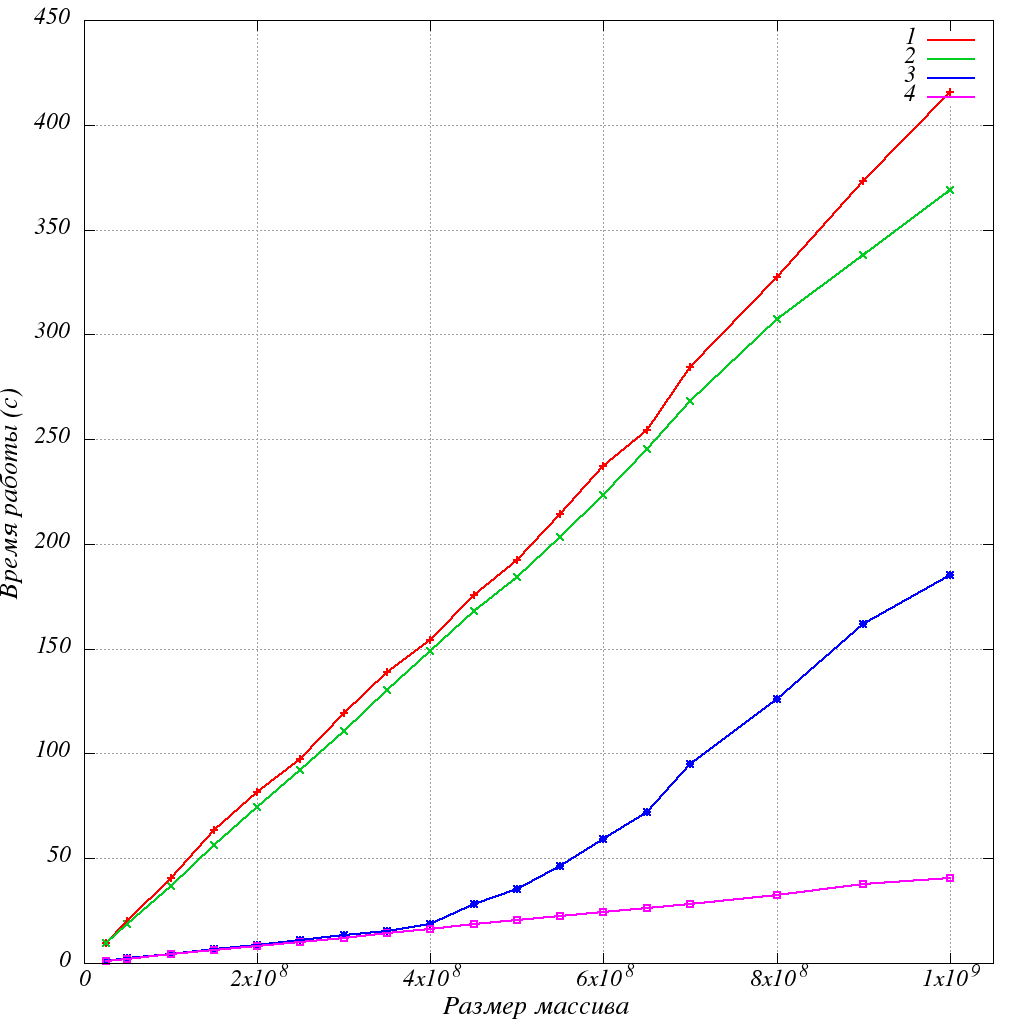
\includegraphics[width=1\linewidth]{graphics.png}}
\caption{
1 -- стандартная печать с записью на диск;
2 -- стандартная печать с записью в разделяемую память;
3 -- алгоритм(?) с записью на диск;
4 -- алгоритм с записью в разделяемую память.} \label{grap}
\end{figure}

Сначала хочется заметить, что стандартная печать не сильно замедляется при записи в диск. 
Все время скорость работы диска была порядка 40--50 Mb/s.
Диск фактически не оказывает никакого существенного влияния на работу.

Из графиков также видно, что при записи в \textit{shared-memory} отношение времени работы стандартного алгоритма и ускоренного постоянно (оба графика -- прямые).
Это значит, что ускорение одинакого на всех данных.

Однако, такого нельзя сказать в случае записи на диск.
На графике в точке $4 \cdot 10^8$ (9.6 GB) происходит излом: начинает ощущаться влияние диска (именно это мы и наблюдали в Тесте 1 -- ускорение немного упало при $5 \cdot 10^8$.)
С этого момента печать начинает упираться в диск.
При запуске тестов было замечено, что скорость записи на диск временами достигает 800-900 Mb/s.
Из-за слишком больших файлов (так файл при размере массива $10^9$ достигает 24 GB) создается очередь из буфферов на печать.
Потоки-обработчики обрабатывают буфферы быстрее, чем производится сама печать.
Разница между третьим и четвертым графиком -- эта время работы диска. 
Эту разницу нельзя ускорить.

\subsection{Тестирование на реальных моделях}
??????????\\
\begin{tabular}{||l||c|c|c||}
\hline
\hline
& Время работы & Время работы & Ускорение \\
\hline
\hline
COORD & 0.028 & 0.003 & 9.33 \\
\hline
ZCORN & 0.135 & 0.013 & 10.38 \\
\hline
COORD & 0.132 &  0.010 & 13.2 \\
\hline
ZCORN & 12.819 & 0.982 & 13.05 \\
\hline
\hline
\end{tabular}


\section{Заключение}
\newpage

\newpage
\begin{thebibliography}{}

\bibitem{1} \textsc{Florian Loitsch}.
Printing Floating-Point Numbers Quickly and Accurately with Integers, 2004.
\bibitem{2} \textsc{Wojciech Mu\l a}.
SSE: conversion integers to decimal representation, 2011.


\end{thebibliography}

\end{document}
